\subsection{Introduction}
\begin{frame}{Dimension Reduction Methods}{Introduction}

\begin{itemize}
    \item We now explore approaches that transform the predictors and then fit an OLS model using the transformed variables. \pause 

    \item Let $Z_1 , Z_2 , \cdots , Z_M$ represent $M < p$ linear combinations of our original reduction $p$ predictors. That is, \pause 

    \begin{equation}\label{eq:z-combs}
        Z_m = \sum_{j=1}^p \phi_{jm} X_j
    \end{equation} \pause 

    for some constants $\phi_{1m} , \phi_{2m} \cdots , \phi_{pm} , m = 1, \cdots , M$ . \pause We can then fit the model $y_i$ using OLS. \pause 

    \begin{equation}\label{eq:linear_dim}
        y_i = \theta_0 + \sum_{m=1}^M \theta_m z_{im} + \epsilon_i, \, \, \, i=1, \cdots, n. 
    \end{equation} \pause 
     
     \item The \textbf{dimension reduction} comes from reducing the problem of estimating the $p + 1$ coefficients $\beta_p$ to estimating the $M + 1$ coefficients $\theta_p$, where $M < p$.
\end{itemize}
    
\end{frame}

\begin{frame}{Dimension Reduction Methods}{Introduction}

Notice that from (\ref{eq:z-combs}), \pause 

\begin{equation*}
    \sum_{m=1}^M \theta_m z_{im} = \sum_{m=1}^M \theta_m \sum_{j=1}^p \phi_{jm} x_{ij} = \sum_{j=1}^p \sum_{m=1}^M \theta_m \phi_{jm} x_{ij} = \sum_{j=1}^p \beta_j x_{ij}, 
\end{equation*} \pause 
    where
    \begin{equation}\label{eq:beta-constrain}
        \beta_j = \sum_{m=1}^M \theta_m \phi_{jm}
    \end{equation} \pause 

\begin{itemize}
%    \item Dimension reduction serves to constrain the estimated $\beta_j$ coefficients, since now they must take the form (\ref{eq:beta-constrain}) \pause 

    \item Where $p \gg n$, selecting $M \ll p$ can significantly reduce the variance of the fitted coefficients. \pause 

    \item If $M = p$, and all the $Z_m$ are linearly independent, then (\ref{eq:beta-constrain}) poses no constraints. $\rightarrow$ OLS. \pause 

    \item The selection of the $\phi_{jm}$'s, can be achieved in different ways: \pause 

    \begin{enumerate}
        \item Principal components. \pause 
        \item Partial least squares. 
    \end{enumerate}
\end{itemize}

    
\end{frame}

\subsection{Principal Component Regression}
\begin{frame}{Dimension Reduction Methods}{Principal Component Analysis (PCA)}

Let's define what is \textbf{PCA} \pause 

\begin{itemize}
    \item PCA is a technique for reducing the dimension of an $n \times p$ data matrix $X$. \pause 

    \item The \textit{first PC} $(Z_1)$ direction of the data is that along which the observations \textit{vary the most}. \pause  \\
    $\rightarrow$ If we protect the $n$-observations onto this FP direction, then the resulting projected observations would have the largest variance. \pause 

    \item In general, one can construct up to $p$ distinct PC. \pause 
        
    \item The second PC $Z_2$ is a linear combination of the variables that is uncorrelated with $Z_1$ , and has largest variance subject to this constraint. \pause 

    \begin{figure}
        \centering
        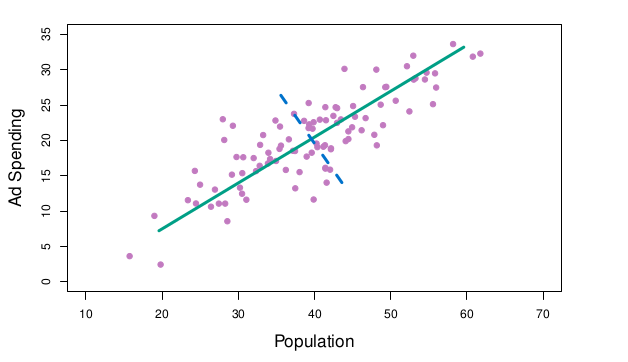
\includegraphics[height=3.5cm]{dim-reduction/pca.png}
    \end{figure} \pause 

\end{itemize}
    
\end{frame}

\begin{frame}{Dimension Reduction Methods}{Principal Component Regression (PCR)}
    \begin{itemize}

    \item The PCR approach involves construct the first $M$ principal components, $Z_1 , \cdots , Z_M $, and then using them as the predictors in a OLS model. \pause 

    \item The key idea is that small number of PC suffice to explain most of the variability in the data, as well the relationship with $Y$. \pause 

    \item In other words, we \textbf{assume} that the directions in which $X_1 , \cdots , X_p$ show the most variation are the directions that are associated with $Y$. \pause 

    \item If the assumption holds, then fitting a OLS model to $Z_1 , \cdots , Z_M $ will lead to better results than fitting a OLS to $X_1 , \cdots , X_p$. \pause 

    \item The number of PC, $M$, is typically chosen by cross-validation. \pause 
    \end{itemize}


    \begin{block}{Note}

    \begin{itemize}
        \item These PC directions are identified in an \textcolor{blue}{unsupervised way}. \pause \\
        $\rightarrow Y$ does not supervise the identification of the PC. \pause 
        \\ 

        \item There is no guarantee that the directions that best explain the predictors will also be the best directions to use for predicting $Y$.
    \end{itemize}
        
    \end{block}
    

    
\end{frame}

\subsection{Partial Least Squares}
\begin{frame}{Dimension Reduction Methods}{Partial Least Squares}

    \begin{itemize}
        \item PLS is a \textcolor{blue}{supervised} alternative to PCR. \pause 

        \item  We first identify  $Z_1 , \cdots , Z_M$ and then fit an OLS model using these $M$ new features. \pause 
    \end{itemize}

\textbf{How PLS compute first directions: } \pause 

Recall the equation (\ref{eq:z-combs}), \pause 

\begin{equation*}
    Z_m = \sum_{j=1}^p \phi_{jm} X_j
\end{equation*} \pause 

\begin{enumerate}
    \item Standardize $p$ predictors. \pause 
    \item Computes $Z_1$ by setting each $\phi_{j1}$ in (\ref{eq:z-combs}) equal to the coefficient from the simple linear regression of $Y$ onto $X_j$. \\ \pause 
    $\rightarrow$ $Z_1 = \beta_1 = X_j^T(y - \beta_0)$ \pause 
\end{enumerate}

\begin{itemize}
    \item In fact, this coefficient is proportional to the correlation between $Y$ and $X_j$. \pause 
    
    \item PLS places the highest weight on the variables that are most strongly related to $Y$.

    
    
\end{itemize}


\end{frame}

\begin{frame}{Dimension Reduction Methods}{Partial Least Squares}

\textbf{To identify the second PLS direction:}

    \begin{enumerate}
        \item We make a regression of each variable on $Z_1$ and take the residuals. \pause 
        
        \item These residuals can be interpreted as the \textit{remaining information} that has not been explained by the first PLS direction. \pause 
        
        \item We then compute $Z_2$ using this orthogonalized data in exactly the same fashion as $Z_1$ was computed based on the original data. \pause 
    \end{enumerate}


$\rightarrow$ This iterative approach can be repeated $M$ times to identify multiple PLS components $Z_1 , \cdots , Z_M $. \\ \pause 


$\rightarrow$ Finally, we use OLS to predict $Y$ using $Z_1 , \cdots , Z_M $ in exactly the same fashion as for PCR. \\ \pause 

$\rightarrow$ The number $M$ of PLS directions used is a tuning parameter that is typically chosen by cross-validation.

    
\end{frame}